\documentclass[tikz]{standalone}
\usepackage{siunitx}
\usetikzlibrary{decorations.pathmorphing,patterns,calc}

\tikzset{
  spring/.style={
    decoration={aspect=0.3, segment length=#1, amplitude=0.4mm,coil},
    decorate
  },
  spring/.default=3pt
}

\begin{document}
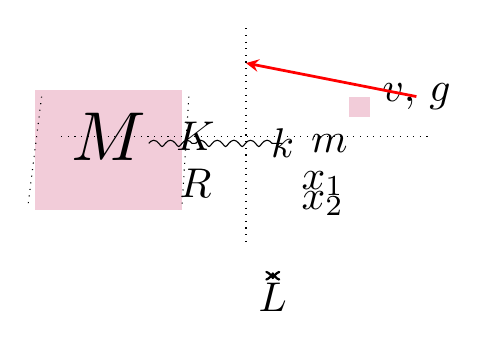
\begin{tikzpicture}[scale=0.85]
  \fill[purple!20] (1.8,0) rectangle (4,1.8);
  \node[scale=2.5] at (2.9,1.1) {$M$};

  \draw[dotted,line width=0.4pt] ($(current bounding box.north east)+(0.1,-0.1)$) -- ($(current bounding box.south east)-(0.1,-0.1)$);
  \draw[dotted,line width=0.4pt] ($(current bounding box.north west)+(0.1,-0.1)$) -- ($(current bounding box.south west)-(0.1,-0.1)$);

  \node[scale=1.5] at (5.5,1) {$k$};
  \draw[spring=6pt] (4.2,1) -- (5.5,1);
  
  \node[scale=1.5] at (6.2,1) {$m$};
  \node[scale=1.5] at (6.5,1.8) {};
  \fill[purple!20] (6.5,1.7) rectangle (6.8,1.4);
  \node[scale=1.5] at (7.5,1.7) {$v$, $g$};
  \draw[-stealth,line width=1pt,red] (7.5,1.7) -- ($(current bounding box.north)+(0,0.1)$);

  \node[scale=1.5] at (4.2,0.4) {$R$};
  \node[scale=1.5] at (4.2,1.1) {$K$};
  \draw[spring=6pt] (3.5,1) -- (4.2,1);
  
  \draw[dotted,line width=0.4pt] ($(current bounding box.north)+(0,0.5)$) -- ($(current bounding box.south)+(0,-0.5)$);
  \draw[dotted,line width=0.4pt] ($(current bounding box.west)+(0.5,0)$) -- ($(current bounding box.east)+(-0.5,0)$);
  

  \node[scale=1.5] at (6.1,0.4) {$x_{1}$};
  \node[scale=1.5] at (6.1,0.1) {$x_{2}$};
  \draw[<->,line width=1pt] ($(current bounding box.south)+(0.4,-0.4)$) -- ($(current bounding box.south)+(0.4,-0.1)$);
  \node[scale=1.5] at ($(current bounding box.south)+(0.4,-0.25)$) {$L$};
  
\end{tikzpicture}
\end{document}